\section{Informe de Evaluación}

Se realizó una evaluación del prototipo funcional de WebSIS con el propósito de verificar su usabilidad e identificar oportunidades de mejora. La evaluación no se entendió como un cierre, sino como una etapa del proceso iterativo de Diseño Centrado en el Usuario: los problemas detectados se corrigieron sobre el propio prototipo y se verificó el resultado.

\subsection{Metodología de evaluación}

Las técnicas de pruebas de usabilidad y evaluación heurística permitieron analizar la interacción de los usuarios con el prototipo, identificando fortalezas, problemas de usabilidad y oportunidades de mejora en la interfaz.

\subsubsection{Pruebas de usabilidad}

Se realizaron pruebas con tres estudiantes de la Facultad de Ciencias y Tecnología: un ingresante y dos regulares. Los participantes ejecutaron las siguientes tareas:

\begin{itemize}
  \item Verificar el estado de matrícula.
  \item Localizar una materia específica para inscripción.
  \item Consultar el Kardex académico.
  \item Identificar el estado de una materia cursada.
\end{itemize}

Se registró el tiempo de ejecución, las dudas manifestadas y los errores cometidos durante cada tarea.

\subsubsection{Evaluación heurística}

Se realizó una inspección heurística utilizando las diez heurísticas de Nielsen (1994). Cada problema identificado fue clasificado según la heurística afectada y su nivel de severidad.

\subsection{Problemas encontrados}

Se identificaron tres problemas durante la evaluación. Los tres fueron detectados tanto en las pruebas de usabilidad como en la evaluación heurística, lo que refuerza su validez.

\renewcommand{\arraystretch}{1.35}
\begin{table}[H]
\centering
\small
\begin{tabularx}{\textwidth}{|c|c|X|l|l|c|}
\hline
\textbf{ID} & \textbf{Técnica} & \textbf{Descripción} & \textbf{Módulo} & \textbf{Perfil} & \textbf{Frec.} \\
\hline
P-01 & PU + HE & El estado de matrícula, mostrado como \textit{Pago registrado}, tenía bajo contraste tanto en modo claro como en modo oscuro, lo que dificultaba su lectura a primera vista. & Estado de matrícula & Ambos & 3/3 \\
\hline
P-02 & PU + HE & Las abreviaturas de estado del Kardex, como APR, REP y ABA, no contaban con una leyenda de referencia. Dos evaluadores no reconocieron \textit{ABA} de forma inmediata. & Kardex & Ingresante & 2/3 \\
\hline
P-03 & PU + HE & El módulo de inscripción permitía seleccionar dos materias cuyos horarios se solapan sin advertir el conflicto. El estudiante solo descubría el choque al revisar su horario, ya finalizada la inscripción. & Inscripción a materias & Ambos & 3/3 \\
\hline
\end{tabularx}
\caption{Problemas identificados durante la evaluación del prototipo.}\label{tab:eval-problemas}
\end{table}
\renewcommand{\arraystretch}{1}

\noindent\textit{Nota.} PU corresponde a pruebas de usabilidad, HE corresponde a evaluación heurística y Frec. indica la frecuencia observada entre los participantes o evaluadores.

\vspace{0.5cm}
\begin{figure}[H]
    \centering
    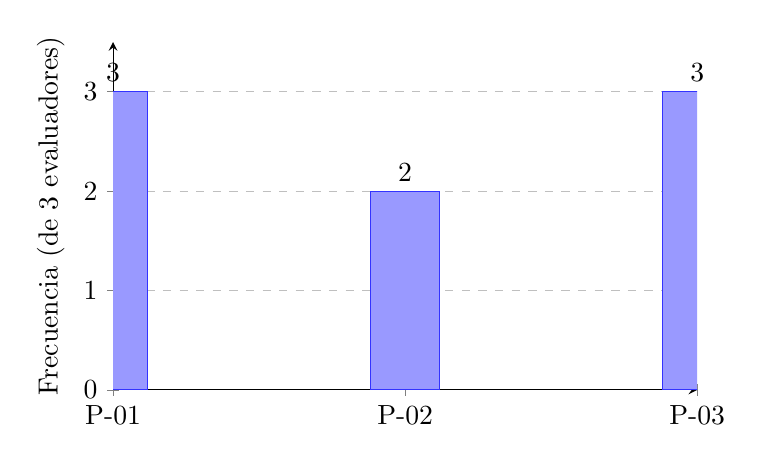
\begin{tikzpicture}
    \begin{axis}[
        ybar,
        enlargelimits=0.2,
        ylabel={Frecuencia (de 3 evaluadores)},
        symbolic x coords={P-01, P-02, P-03},
        xtick=data,
        nodes near coords,
        nodes near coords align={vertical},
        ymin=0, ymax=3.5,
        bar width=25pt,
        width=9cm,
        height=6cm,
        axis x line=bottom,
        axis y line=left,
        ymajorgrids=true,
        grid style=dashed,
    ]
    \addplot[fill=blue!40, draw=blue!80] coordinates {(P-01,3) (P-02,2) (P-03,3)};
    \end{axis}
    \end{tikzpicture}
    \caption{Frecuencia de detección de cada problema durante la evaluación.}
    \label{fig:frecuencia-problemas}
\end{figure}
\subsection{Nivel de severidad}

Se utilizó la escala de severidad de Nielsen (1994): 0 = no es problema; 1 = cosmético; 2 = menor; 3 = moderado; 4 = catastrófico.

\renewcommand{\arraystretch}{1.35}
\begin{table}[H]
\centering
\small
\begin{tabularx}{\textwidth}{|c|p{2.6cm}|p{2.6cm}|l|X|}
\hline
\textbf{ID} & \textbf{Problema} & \textbf{Heurística} & \textbf{Severidad} & \textbf{Justificación} \\
\hline
P-01 & Bajo contraste del estado de matrícula en modo claro y oscuro. & H1 -- Visibilidad del estado del sistema. & 2 -- Menor & El estado de matrícula es información crítica para habilitar la inscripción. Si el estudiante no lo identifica con claridad, puede iniciar el proceso sin saber si está habilitado. No bloquea la tarea, pero genera incertidumbre. \\
\hline
P-02 & Abreviaturas del Kardex sin leyenda, como APR, REP y ABA. & H2 -- Coincidencia con el mundo real. & 2 -- Menor & \textit{ABA} no forma parte del vocabulario cotidiano del estudiante. Sin leyenda visible, el usuario debe inferir su significado. \\
\hline
P-03 & La inscripción no advierte cuando dos materias tienen horarios solapados. & H5 -- Prevención de errores. & 3 -- Moderado & El sistema dejaba registrar materias con choque de horario sin ninguna alerta. El estudiante solo lo detectaba después, al consultar su horario, lo que puede obligarlo a corregir la inscripción en un periodo de tiempo acotado. \\
\hline
\end{tabularx}
\caption{Nivel de severidad de los problemas identificados.}\label{tab:eval-severidad}
\end{table}
\renewcommand{\arraystretch}{1}

El problema P-03 es el de mayor severidad, con nivel 3 -- Moderado, dado que afecta directamente la tarea de mayor criticidad del sistema: una inscripción con horarios solapados que el sistema no previene obliga al estudiante a rehacer parte del proceso. Los problemas P-01 y P-02 son de severidad menor y no impiden la completación de las tareas, pero reducen la claridad y la confianza del usuario.

\subsection{Mejoras aplicadas tras la evaluación}

Coherentemente con el carácter iterativo del Diseño Centrado en el Usuario, los tres problemas detectados se corrigieron directamente sobre el prototipo funcional. La siguiente tabla resume la intervención realizada para cada uno; las figuras posteriores muestran el resultado.

\renewcommand{\arraystretch}{1.35}
\begin{table}[H]
\centering
\small
\begin{tabularx}{\textwidth}{|c|l|X|l|}
\hline
\textbf{ID} & \textbf{Heurística} & \textbf{Mejora aplicada en el prototipo} & \textbf{Estado} \\
\hline
P-03 & H5 -- Prevención de errores. & Se implementó la detección automática de solapamiento de horarios: al seleccionar materias, el sistema compara sus bloques y, si dos se solapan, muestra una alerta que identifica el conflicto y bloquea la finalización de la inscripción hasta resolverlo. & Corregido \\
\hline
P-01 & H1 -- Visibilidad del estado. & Se aumentó el contraste del indicador de estado de matrícula usando fondo sólido y texto de alto contraste, verificando el resultado en modo claro y oscuro. & Corregido \\
\hline
P-02 & H2 -- Coincidencia con el mundo real. & Se agregó una leyenda visible sobre la tabla del Kardex (APR = Aprobada, REP = Reprobada, ABA = Abandonada, En curso) y un texto descriptivo al pasar el cursor sobre cada indicador. & Corregido \\
\hline
\end{tabularx}
\caption{Mejoras aplicadas sobre el prototipo tras la evaluación.}\label{tab:eval-mejoras}
\end{table}
\renewcommand{\arraystretch}{1}

\begin{figure}[H]
  \centering
  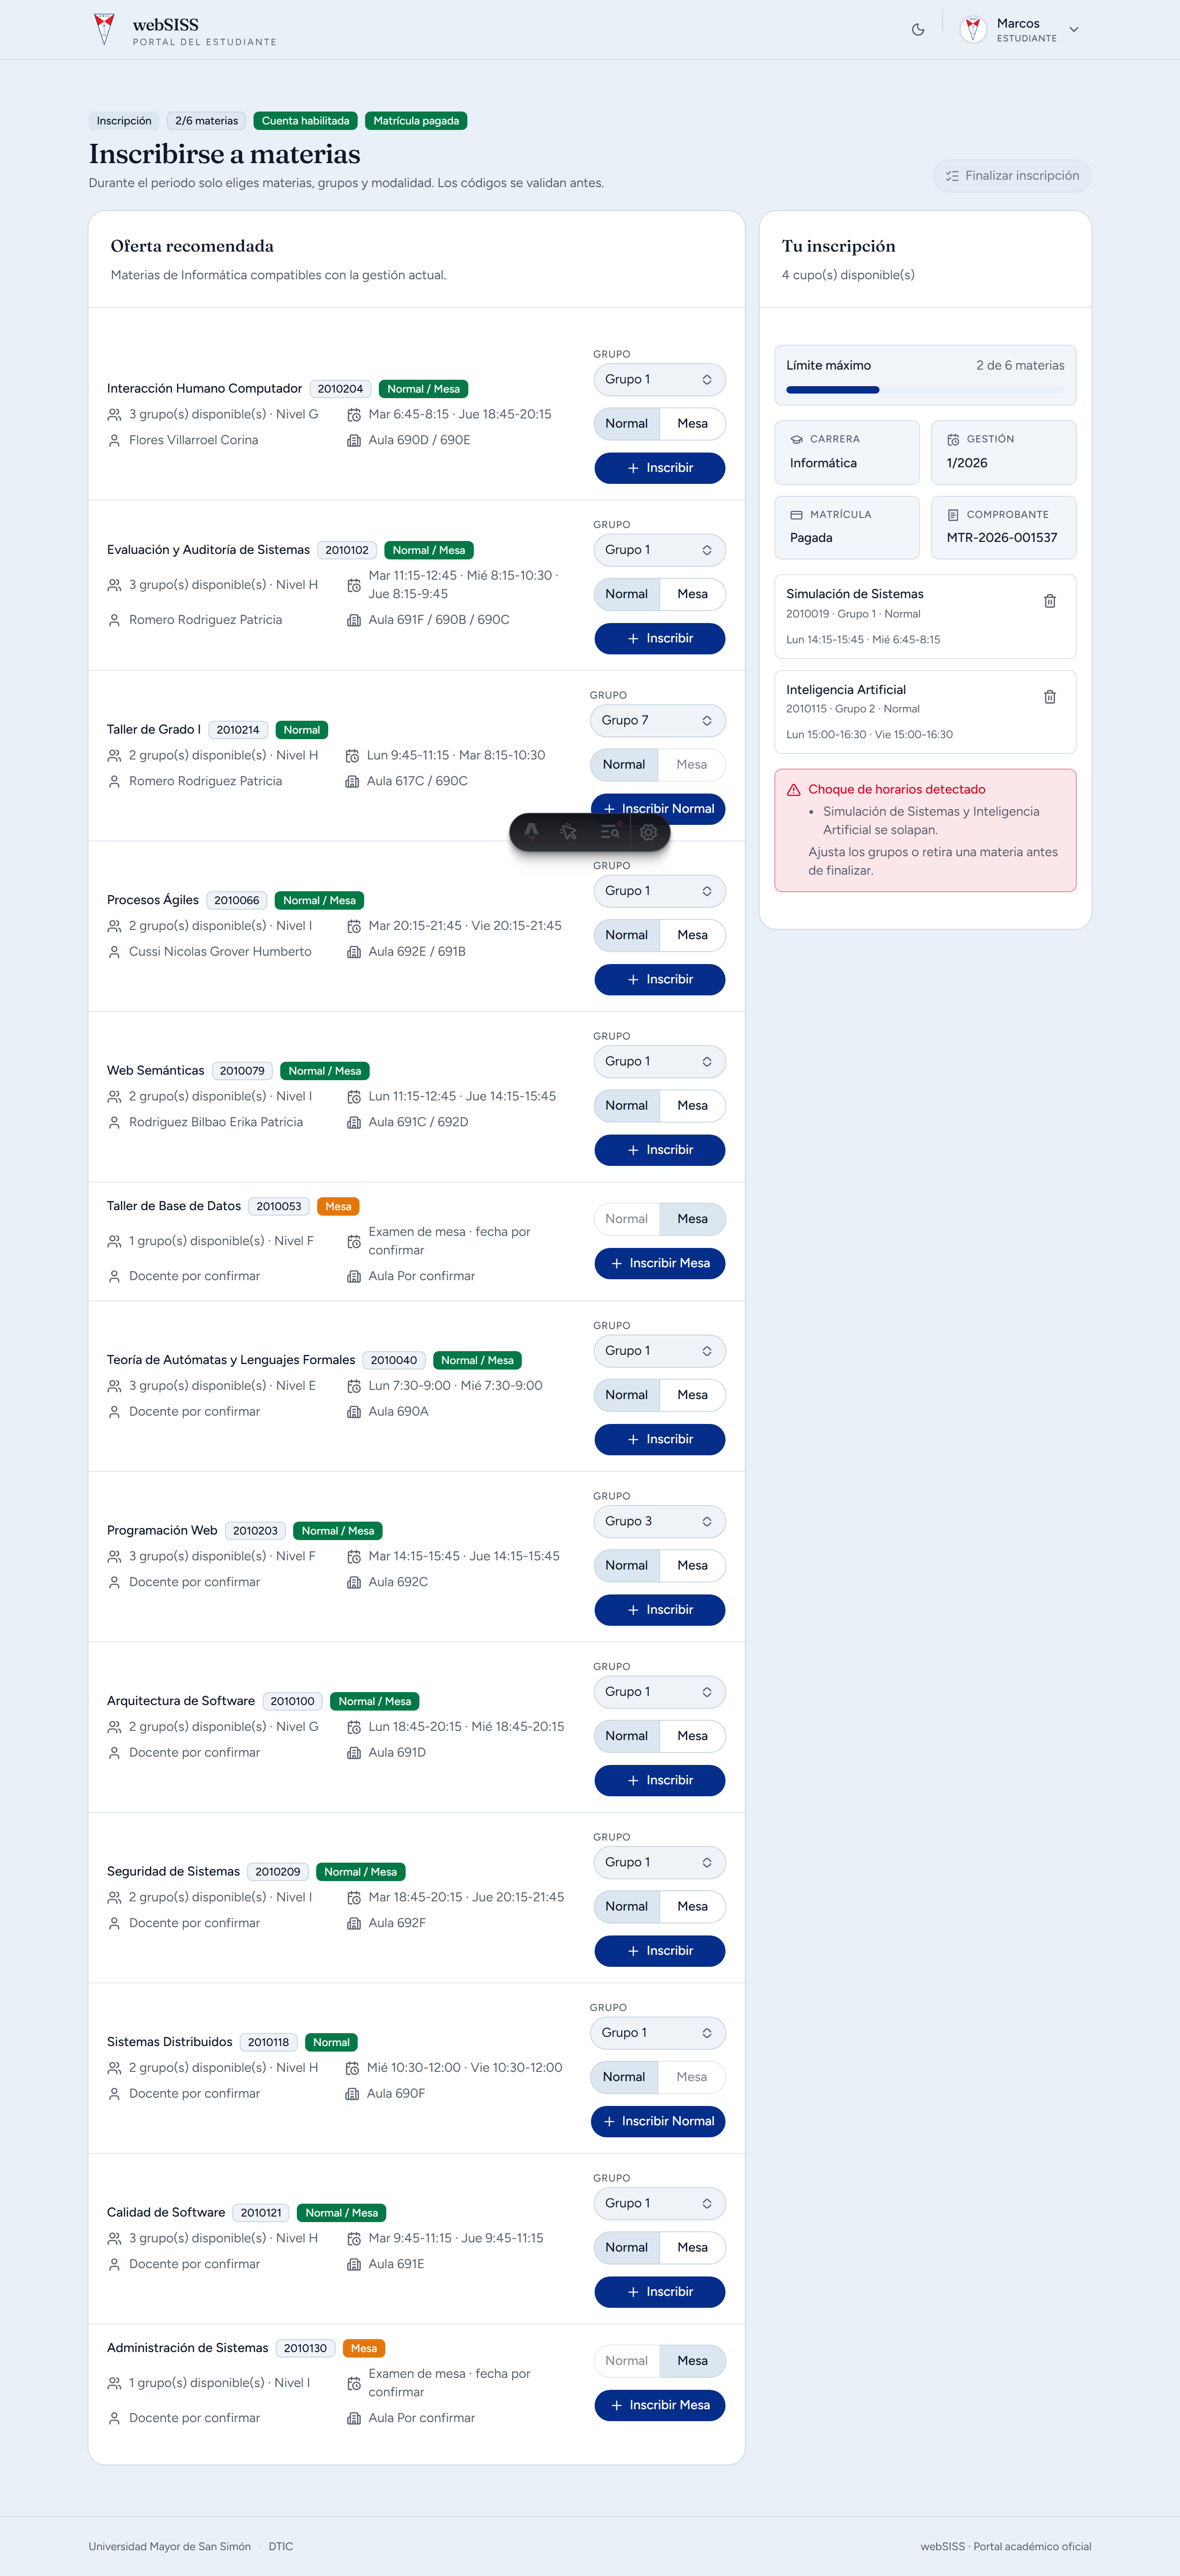
\includegraphics[width=\textwidth,height=0.72\textheight,keepaspectratio]{images/prototipo/10-inscripcion-conflicto.png}
  \caption{P-03 corregido: la inscripción detecta el choque de horarios entre dos materias y bloquea la finalización hasta resolverlo.}
  \label{fig:fix-conflicto}
\end{figure}

\begin{figure}[H]
  \centering
  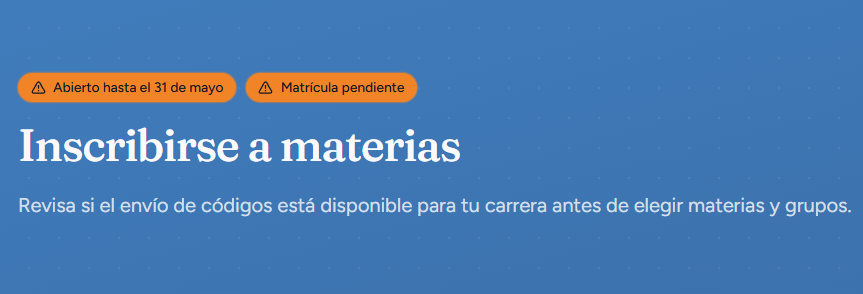
\includegraphics[width=\textwidth,height=0.72\textheight,keepaspectratio]{images/prototipo/13-estado-materia.png}
  \caption{P-01 corregido: el contraste del indicador de estado de matrícula usa fondo sólido y texto de alto contraste, verificado en modo claro y oscuro.}
  \label{fig:fix-estado-matricula}
\end{figure}

\begin{figure}[H]
  \centering
  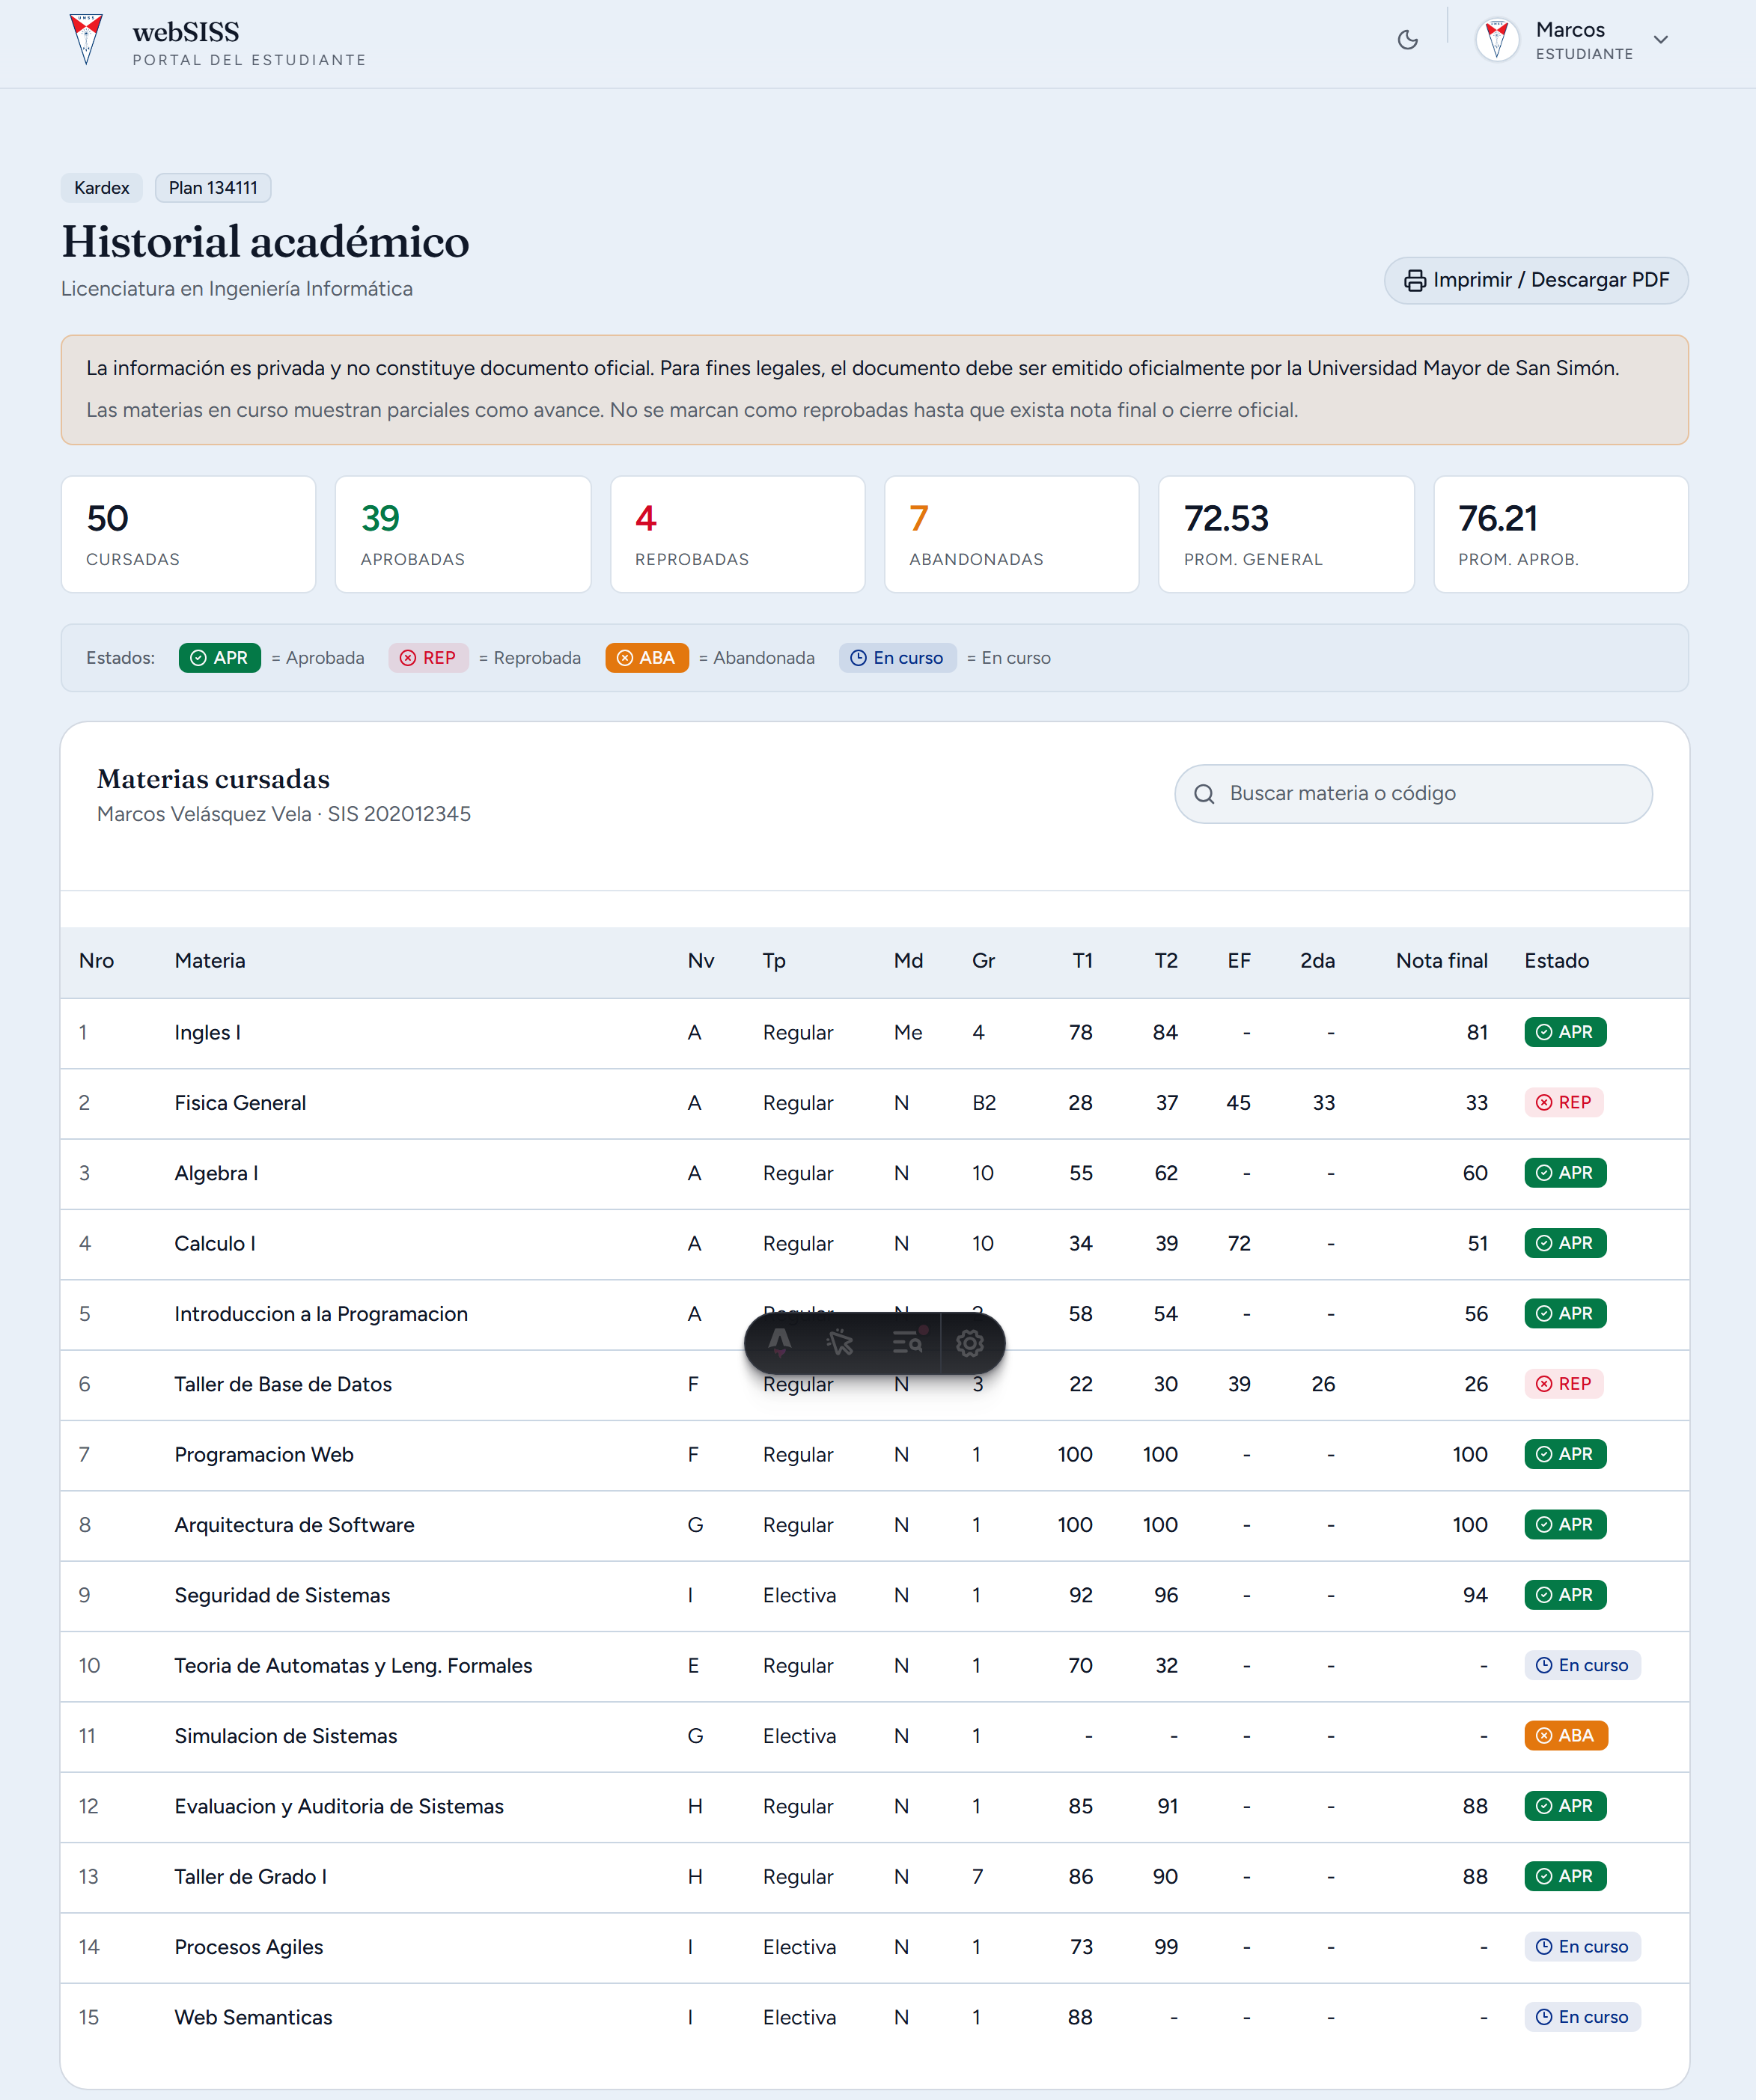
\includegraphics[width=\textwidth,height=0.72\textheight,keepaspectratio]{images/prototipo/08-kardex.png}
  \caption{P-02 corregido: el Kardex incorpora una leyenda visible de las abreviaturas de estado sobre la tabla.}
  \label{fig:fix-leyenda}
\end{figure}

Además de las correcciones derivadas de los tres problemas evaluados, se ajustaron otros detalles detectados durante la revisión del prototipo, en línea con las heurísticas de Nielsen: se diferenció la acción de imprimir el horario de la del Kardex (consistencia), se incorporó una confirmación explícita antes de retirar una materia de la inscripción (control y libertad del usuario, prevención de errores) y se añadió un estado vacío con orientación cuando el estudiante no tiene materias inscritas (retroalimentación). La Figura~\ref{fig:fix-retiro} y la Figura~\ref{fig:fix-vacio} muestran estos dos últimos ajustes.

\begin{figure}[H]
  \centering
  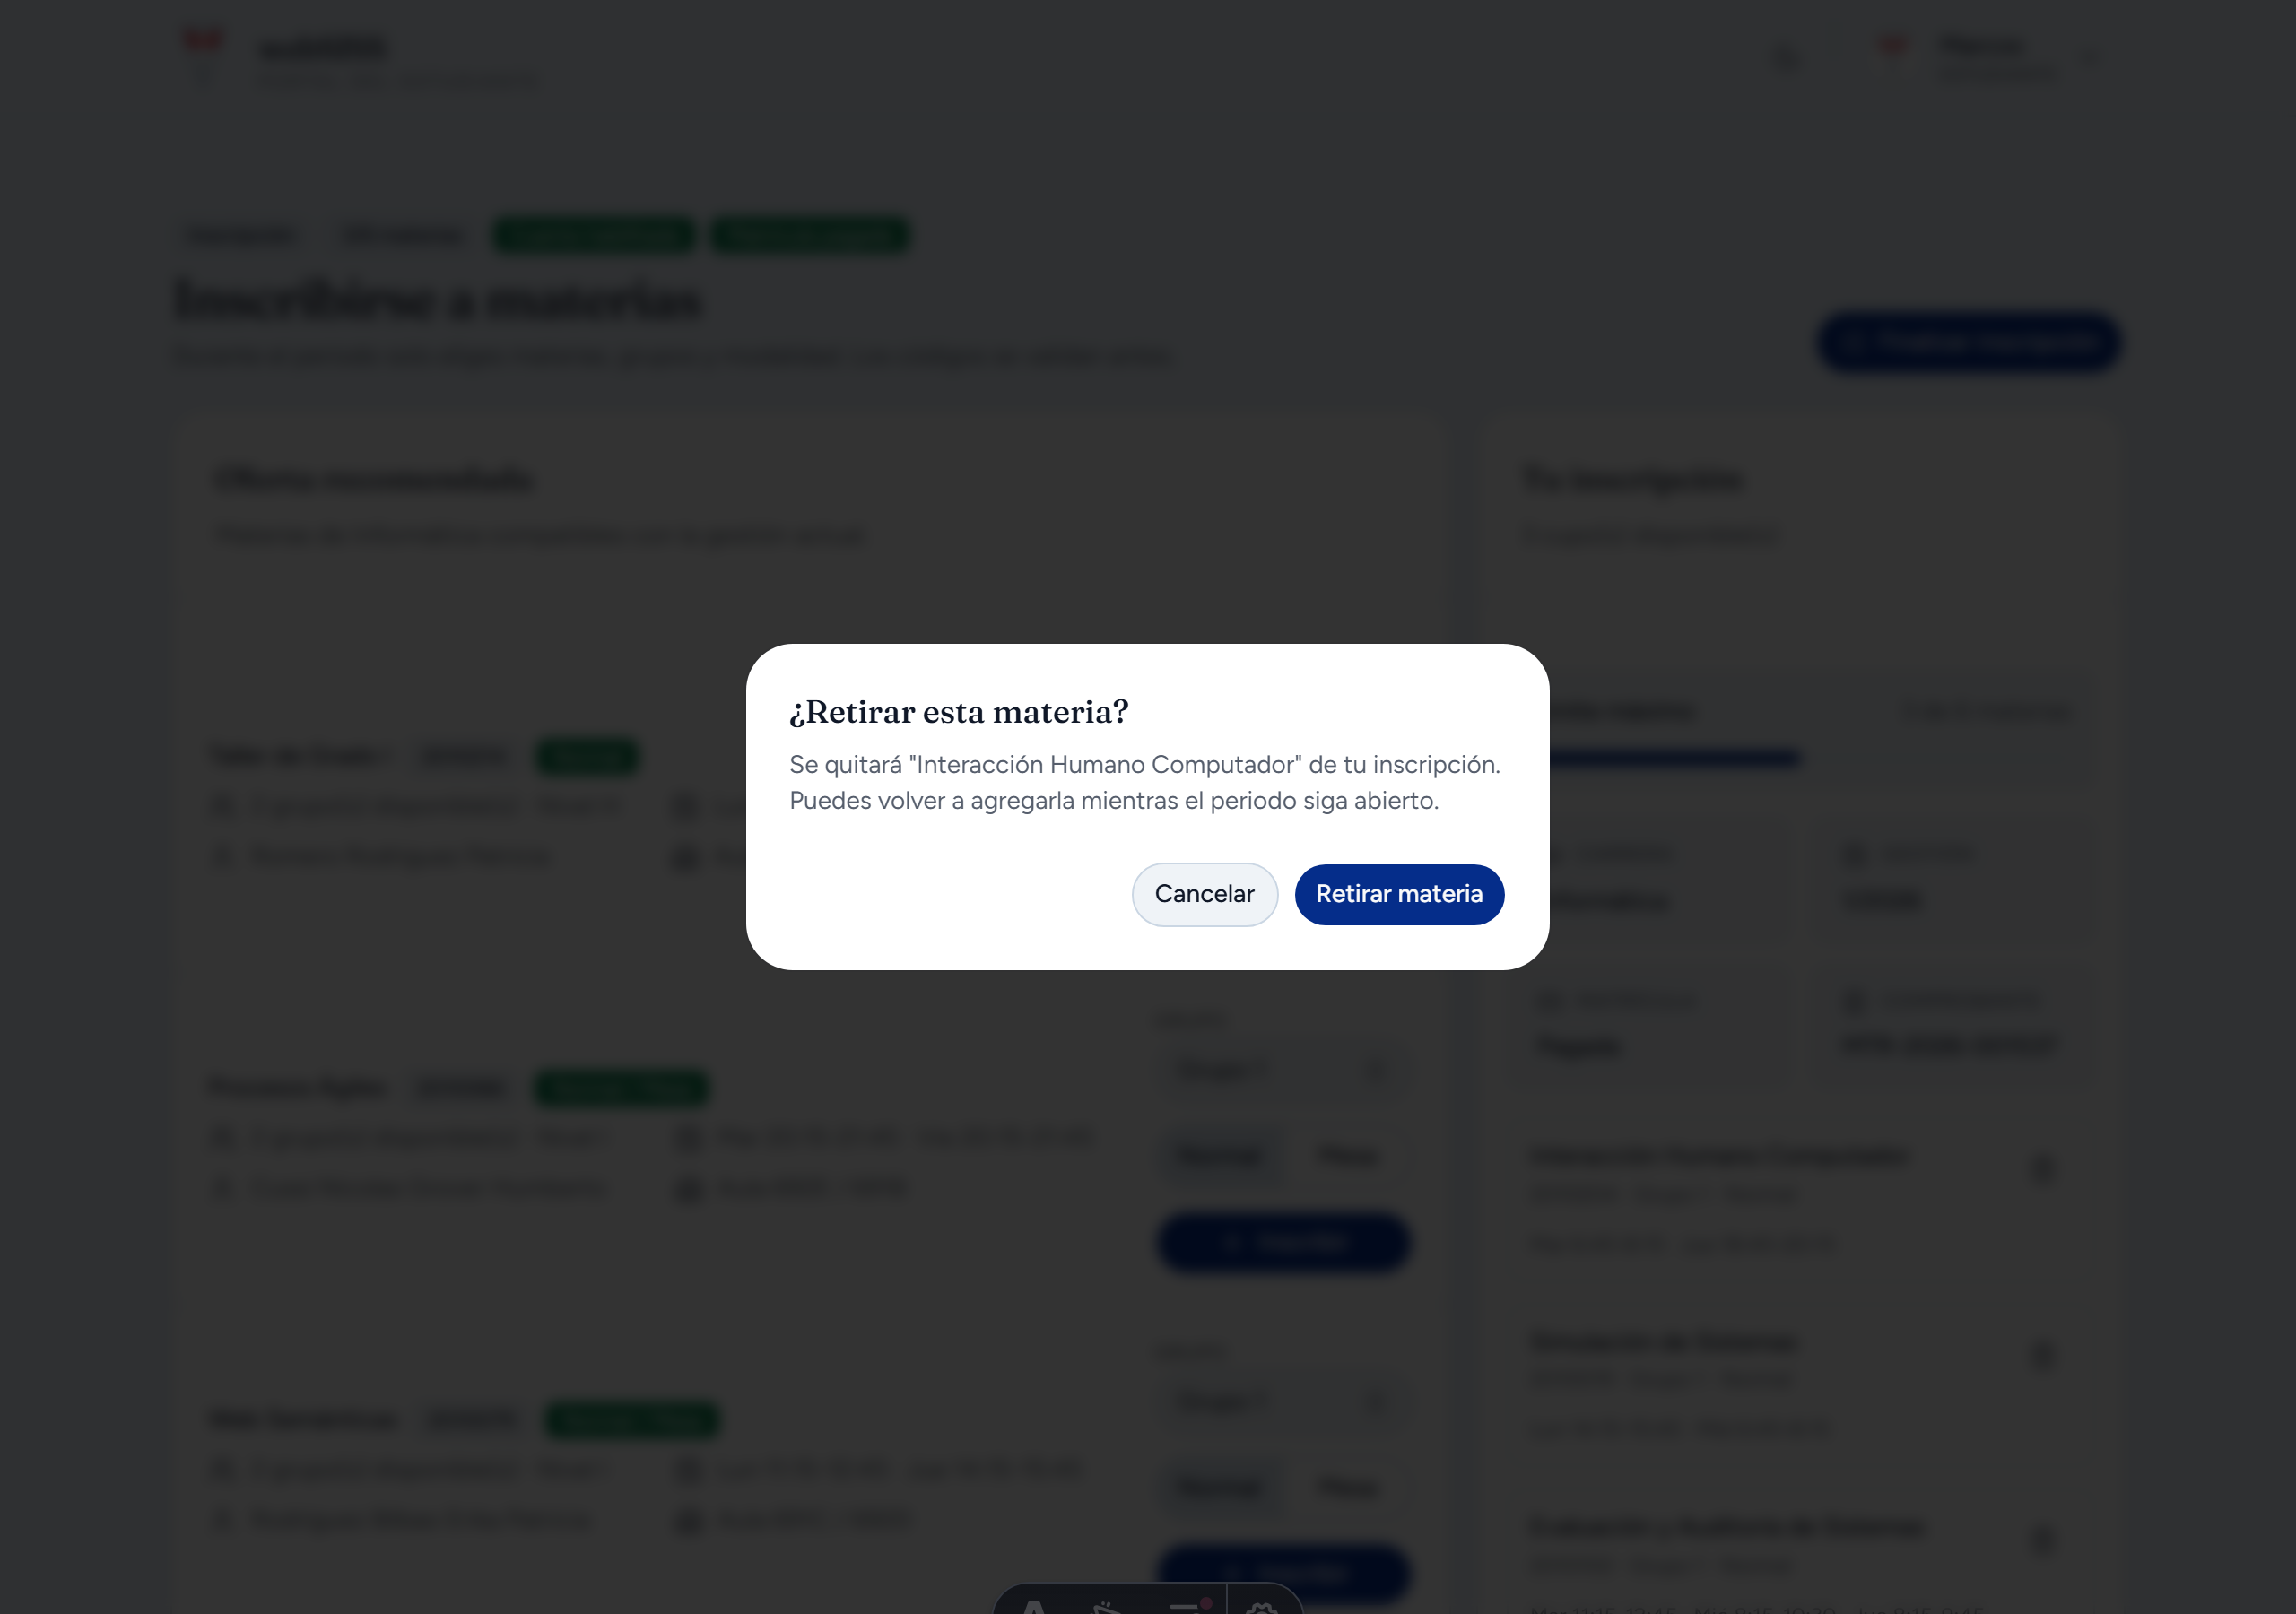
\includegraphics[width=\textwidth,height=0.72\textheight,keepaspectratio]{images/prototipo/12-retiro-confirmacion.png}
  \caption{Confirmación explícita antes de retirar una materia de la inscripción, evitando acciones irreversibles accidentales.}
  \label{fig:fix-retiro}
\end{figure}

\begin{figure}[H]
  \centering
  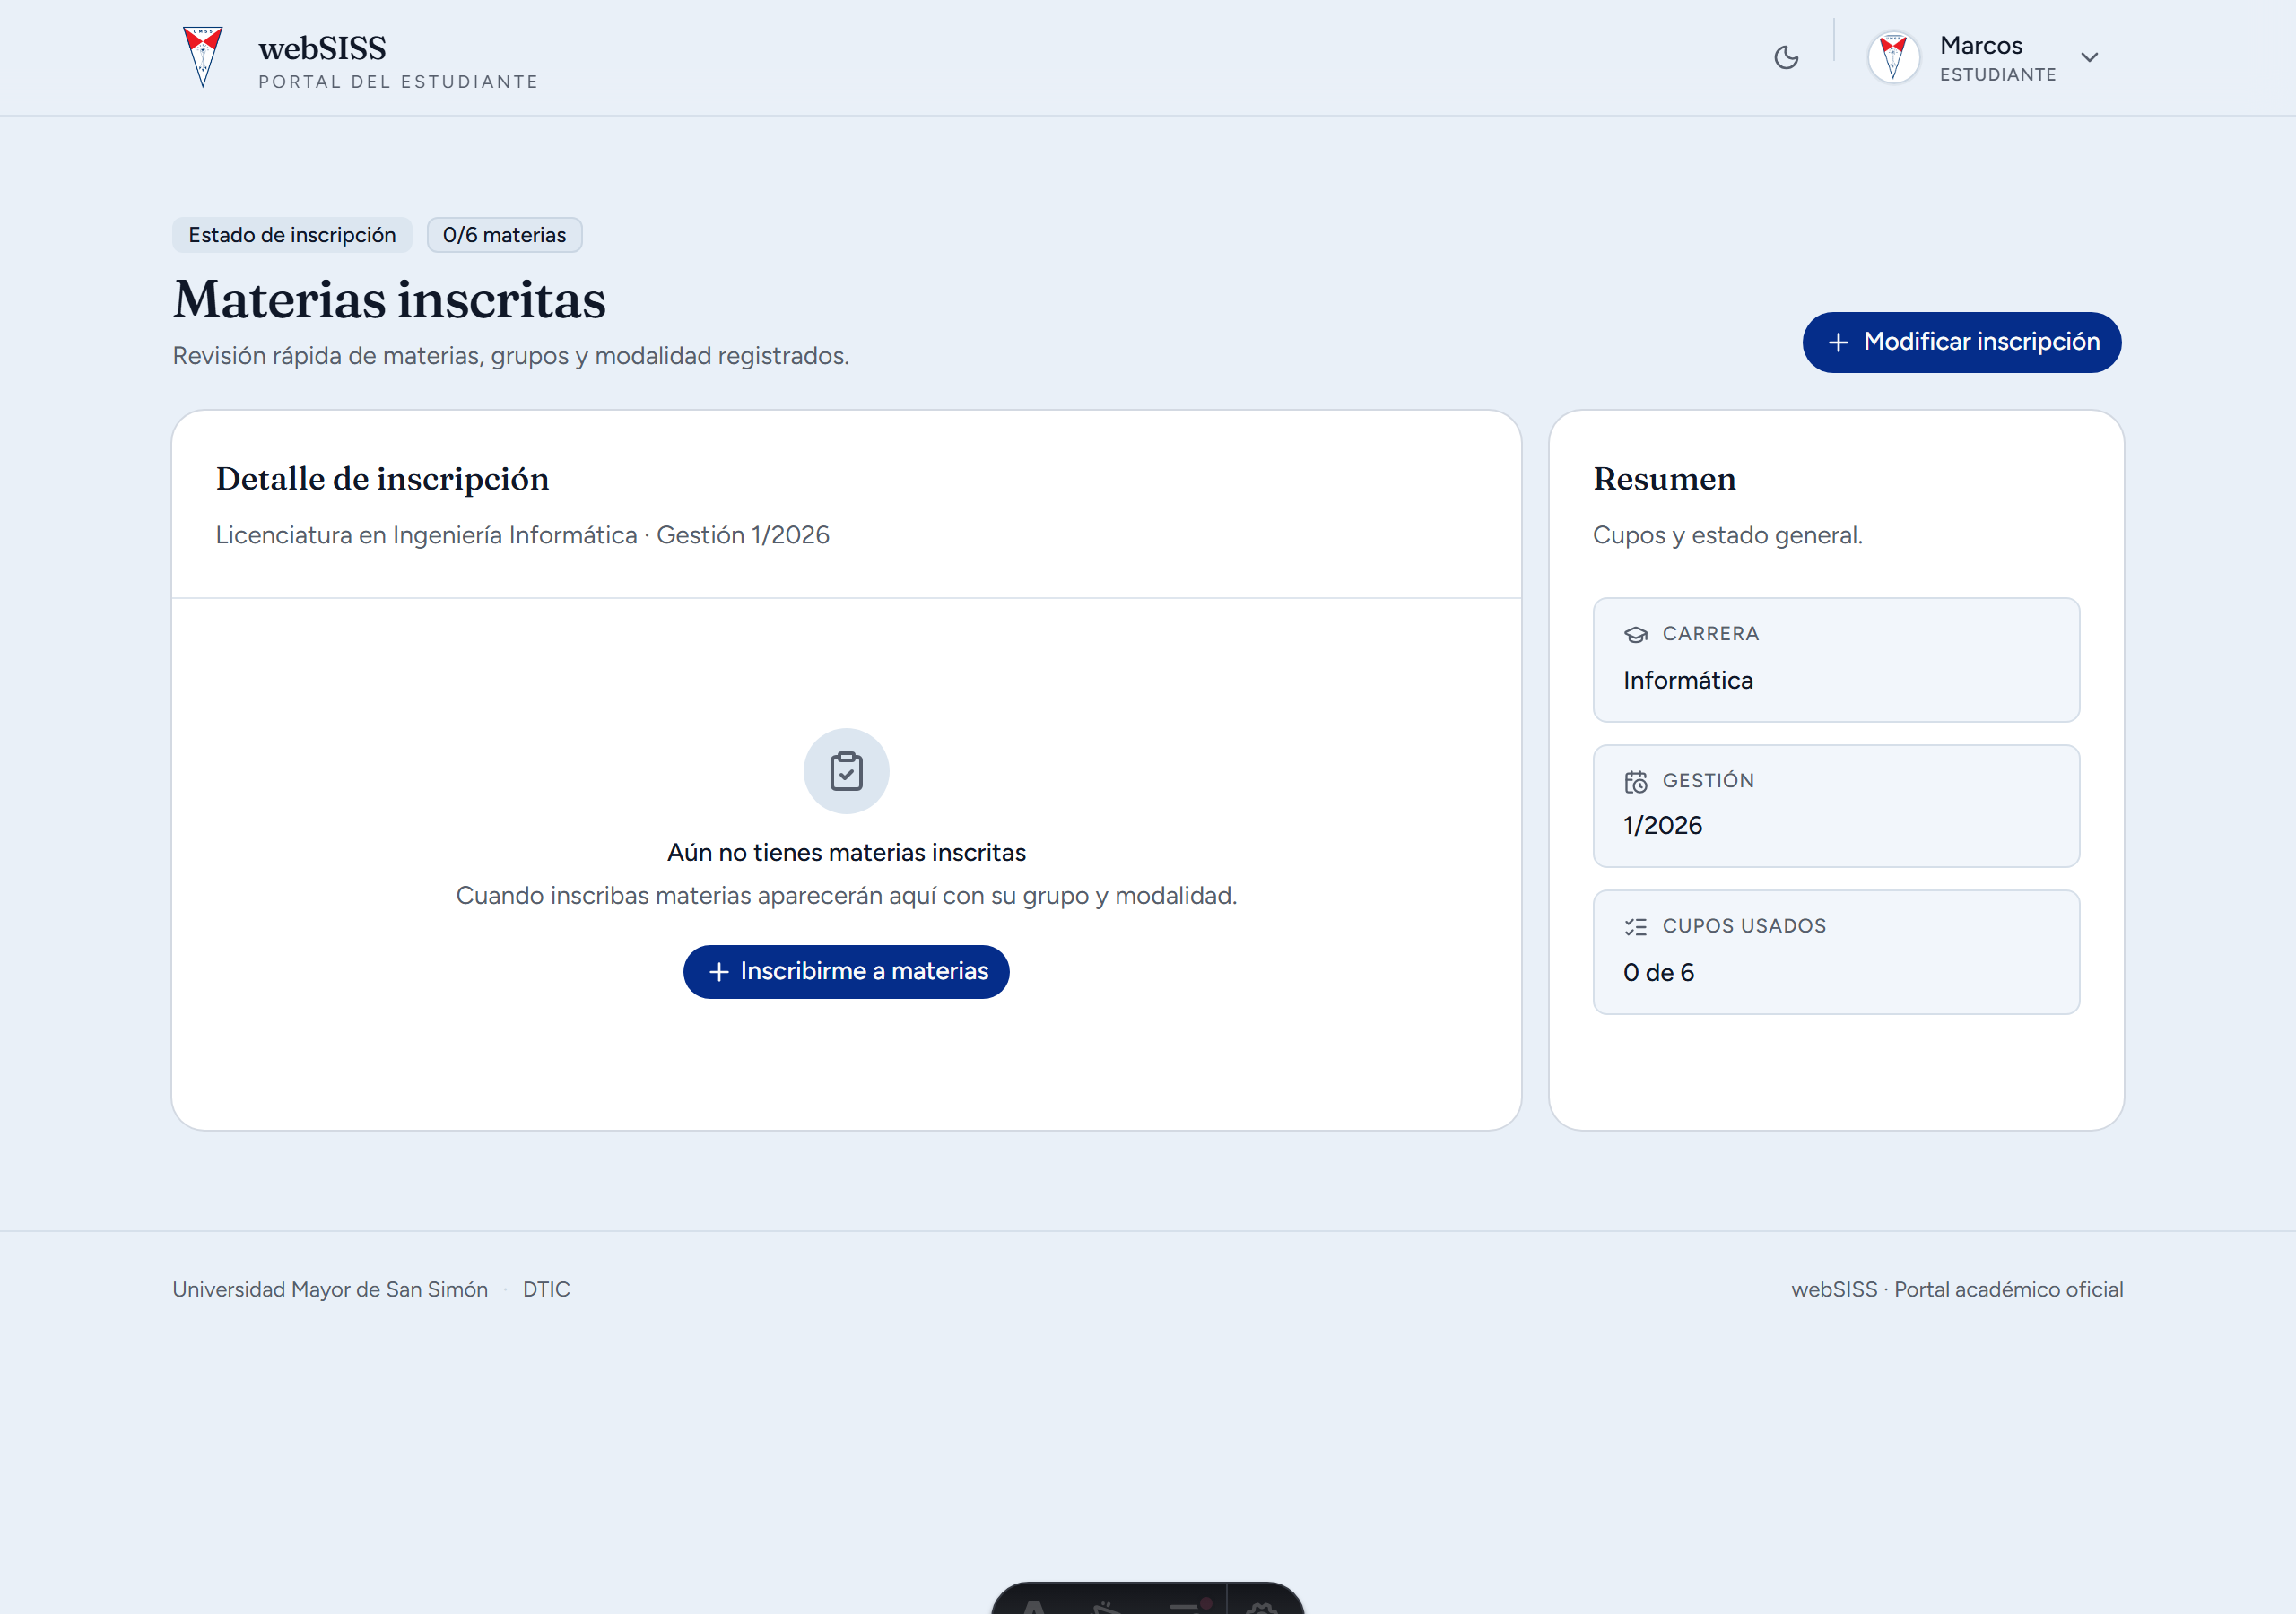
\includegraphics[width=\textwidth,height=0.72\textheight,keepaspectratio]{images/prototipo/11-estado-vacio.png}
  \caption{Estado vacío del módulo de inscripción, con mensaje orientativo y acceso directo para inscribirse.}
  \label{fig:fix-vacio}
\end{figure}

Tras aplicar estas mejoras, los problemas de severidad moderada y menor detectados en la evaluación quedaron resueltos sobre el prototipo, completando un ciclo de detección, corrección y verificación propio del Diseño Centrado en el Usuario.
